\documentclass[a4paper, 12pt]{article}

\usepackage[left = 3cm, top = 3cm, bottom = 3cm, right = 2cm]{geometry}
\usepackage{graphicx}
\usepackage[spanish,es-tabla]{babel} % Idioma español con tablas
\usepackage{amsmath}
\usepackage{amssymb}
\usepackage{amsfonts}
\usepackage[utf8]{inputenc}         % Para escribir en castellano
\usepackage[T1]{fontenc}
\usepackage{color}
\usepackage{alltt}
\usepackage{times}
\usepackage{setspace}  % Usado para doble espacio, espacio y medio y espacio simple
\usepackage{booktabs}         % Para formar tablas
%\usepackage{longtable}       % Usado para diseñar grandes tablas.
\usepackage{enumerate}
\usepackage[round]{natbib} 
\bibliographystyle{apalike}

\usepackage[x11names,table]{xcolor}

\begin{document}

\begin{center}
 {\bf {\fontsize{14}{16.8}\selectfont UNIVERSIDAD NACIONAL DE TRUJILLO}}     
 
    {\bf{\fontsize{14}{16.8}\selectfont Facultad de Ciencias Físicas y Matemáticas}} 

  {\bf{\fontsize{14}{16.8}\selectfont Escuela Profesional de Informática}}
\end{center}  

\begin{figure}[ht]
\begin{center}

\includegraphics[width=.3\textwidth]{unt}
\end{center}
\end{figure}

\vskip 2cm
\begin{center}
  { \bf {\fontsize{17}{20.4}\selectfont{PREDICCIÓN DE LA RESPUESTA CORRECTA DE UNA PREGUNTA DE OPCIÓN MÚLTIPLE MEDIANTE TÉCNICAS DE APRENDIZAJE NO SUPERVISADO ASOCIADO CON LA EXPERIENCIA.}  } } 
\end{center}   
  \vskip 1cm
  { \bf {\fontsize{17}{20.4}\selectfont{\hspace*{-0.4cm}Nombre de autor: José Vicente Clavo Tafur}}  } 
  \vskip 1cm
  { \bf {\fontsize{17}{20.4}\selectfont{\hspace*{-1cm}Nombre del Asesor: Dr. Jorge Luis Gutierrez Gutierrez}}  } 
\vskip 4cm
\begin{center}    
{\bf {\fontsize{14}{16.8}\selectfont Trujillo - La Libertad
\vskip 0.0cm
\hspace*{-0.2cm} 
\vskip 0.1cm
2018 }}
\end{center} 
\newpage

\begin{center}
%\onehalfspace  \doublespacing  \singlespace
\Large {PROYECTO DE INVESTIGACIÓN PARA TRABAJO DE GRADUACIÓN \\
\vskip 0.2cm
 ESCUELA PROFESIONAL DE INFORMÁTICA}
\end{center}
\vskip 1cm

\section{GENERALIDADES}

\subsection{Título}
Predicción de la respuesta correcta de una pregunta de opción múltiple mediante técnicas de aprendizaje no supervisado asociado con la experiencia.

\subsection{Autor(es)}
\begin{table}[h!]
 \caption{\small{Datos del alumno investigador}}
\begin{tabular}{llrrr} \toprule
{\bf Código(s)} & {\bf Nombres y Apellidos} & {\bf Cargo en el proyecto} & {\bf Email} \\ \midrule
xxxxxxxx-xx & José V. Clavo Tafur & Estudiante invest. & jclavotafur@gmail.com           \\
\end{tabular}
\end{table}



\subsection{Tipo de investigación}
\subsubsection{De acuerdo al fin que se persigue (Básica/Aplicada):} 

{\bf Básica:} También denominada pura o fundamental, busca el progreso científico, incrementa los conocimientos teóricos, sin interesarse en las posibles aplicaciones o consecuencias prácticas; es mas formal y persigue las generalizaciones con vistas al desarrollo de una teoría basada  en principios y leyes.\par
\vskip 0.3cm
{\bf Aplicada:} Tiene relación con la investigación básica, pues depende de los descubrimientos y avances de la investigación básica y se enriquece de ellos, pero se caracteriza por su interés en la aplicación, utilización y consecuencias prácticas de los conocimientos. 
%La investigación aplicada busca el conocer para hacer, para actuar, para construir y para modificar.
                
\subsubsection{De acuerdo al alcanze de  la investigación:}
Investigaciones cuantitativas, segun el nivel de asociación de las variables principales \cite{Erica}:
\begin{enumerate} 
\item [a)] {\bf Explicativa o causal}: Consiste en la manipulación de una (o más) variable experimental no comprobada, en condiciones rigurosamente controladas, con el fin de describir de qué modo o por qué causa se produce una situación o acontecimiento particular. El experimento provocado por el investigador le permite introducir determinadas variables de estudio manipuladas por él, para controlar el aumento o disminución de esas variables y su efecto en las conductas observadas. Su método es cuantitativo y su fin es el descubrimiento de las causas.  
\vskip 0.3cm
\item[b)] {\bf Exploratorio}: Es un estudio inicial (examinar un tema poco estudiado) de un fenómeno, normalmente buscando un primer conocimiento del mismo; por ejemplo, cuáles son los aspectos y variables más significativos del fenómeno; y los resultados se consideran provisionales y la base para investigaciones posteriores.
\vskip 0.3cm
\item[c)]{\bf Descriptivo}: Busca describir (frecuencias, porcentajes, medias, etc.) sin relacionarlas inferencialmente, las variables del fenómeno que se estudia. Se situa en el presente, pero no solamente se limita a la simple recolección y tabulación de datos, sino que hace la interpretación y el análisis imparcial de los mismo.  
\vskip 0.3cm
\item[d)] {\bf Correlacional o asociativa}: Busca determinar qué cambios de unas variables están asociados (correlacionados) con cambios en otras variables, normalmente sin establecer relaciones de causalidad, como sí es el caso en los análisis estructurales.
\end{enumerate}


\subsection{Área y línea de Investigación}
\subsubsection{Área de investigación :} 
Ejemplo: Algoritmos y complejidad.
 
\subsubsection{Línea de Investigación:} 
Ejemplo: Estrategias algoritmicas.
               
\subsubsection{Tema de investigación :} qwqwqqwq


\subsection{Localidad e Institución donde se desarrollará el proyecto }
  
\subsubsection{Localidad (Dirección, Distrito, Provincia, Departamento) :} 
\subsubsection{Institución (Universidad/Facultad/Departamento):}

  
\subsection{Duración del trabajo de graduación (Plan TG y desarrollo del TG)}
%Ejemplo:\\
\hspace*{0.7cm}Del \hspace*{0.2cm}04/02/2019 \hspace*{0.3cm} AL\hspace*{0.2cm}28/06/2019  \hspace*{0.2cm}(4. meses +  25. días)
  
      
\subsection{Cronograma del trabajo de graduación}


%\subsubsection{Cronograma del plan TG y avance del desarrollo TG (un ciclo) }

 \begin{table}[h!]
  \caption{\small{Etapas y actividades para el trabajo de graduación}}
\centering
\begin{tabular}{|p{3cm} |p{4cm} |p{2.2cm} |p{2.6cm} |p{2.3cm}|}  \hline   
\textit{{\bf{Etapas}}} & \textit{{\bf{Actividades/tareas}}} & \textit{{\bf{Fecha inicio}}} & \textit{{\bf{Fecha término}}} & \textit{{\bf{Hs. semanal}}}\\ \hline

Preparación del plan TG. & Elaborar plan TG.\par Aprob. plan TG.  & 05/08/2016\par 20/09/2016 & 05/05/2017\par 05/05/2017 & 4\par 1  \\ \hline

Recopilación de información. & Inv. bibliográfica.\par Instrumentos de medición. & 05/05/2017\vskip 0.5cm \par 05/05/2017  & 05/05/2017\vskip 0.5cm \par 05/05/2017 & 30\vskip 0.5cm\par 25    \\  \hline

Análisis de datos recolectados. & Procesamiento e interpretación de la información. &\vskip 0.2cm 05/05/2017 &\vskip 0.2cm 05/05/2017 & \vskip 0.2cm 10 \\ \hline

Resultados. & Desarrollo de TG segun cronograma. &\vskip 0.2cm 05/05/2017 &\vskip 0.2cm 05/05/2017 & \vskip 0.2cm 10 \\ \hline

Redacción del informe TG.  &Informe N1: Marco teórico y metodología. \par
Informe N2: Propuesta de solución al problema formulado.\par 
Informe N3: Resultados y conclusiones preliminares. &\vskip 0.2cm\par  05/05/2017\par \vskip 1.1cm \par 05/07/2017\par \vskip 0.9cm 05/08/2017 & \vskip 0.2cm\par  05/02/2017\par  \vskip 1.1cm 05/05/2017\par \vskip 0.9cm 05/06/2017 &  \vskip 0.2cm\par 50\par  \vskip 1.1cm\par 93\par \vskip 0.9cm 20                \\  \hline

Recopilación de información adicional para la tesis & Inv. bibliográfica adicional y su interpretación.  & 05/08/2016 & 05/05/2017 & 4  \\ \hline

Pruebas y análisis de resultados & Preparación de resultados finales.  & 05/08/2016 & 05/05/2017 & 4  \\ \hline


Redacción del informe de tesis & Informe de tesis de acuerdo con formato establecido.  & 05/08/2016 & 05/05/2017 & 4  \\ \hline
\end{tabular}
\begin{center}
\vskip -0.2cm
{\small{Fuente: Elaboración propia.}}
\end{center}
\end{table}




\subsection{Recursos disponibles}
\subsubsection{{\bf Personal:}} Personal técnico, administrativo y de servicios disponibles para el proyecto.
\subsubsection{ {\bf	Materiales y Equipos:}} Se debe especificar la calidad y cantidad de equipos, instrumentos y materiales disponibles  para ejecutar el trabajo de investigación.
\subsubsection{{\bf Locales:}} Señalar los ambientes donde se realizará la investigación: laboratorios, aulas, biblioteca, hemeroteca, etc.  indicando su ubicación precisa.

\subsection{Presupuesto}
Costear en nuevos soles, los bienes, servicios e inversiones necesarios para llevar a cabo la investigación y que no estén disponibles. Presentar ordenados de acuerdo a la codificación del  Clasificador de Gastos vigente. Considerar calidad, cantidad y  precio.

\subsection{Financiamiento}
\subsubsection{ {\bf	Con recursos universitarios:}}  Los recursos disponibles por subvención por investigación.
\subsubsection{ {\bf Con recursos externos:}} Los que se perciban de fuente distinta a la UNT. Indicar la entidad aportante y los montos.
\subsubsection{ {\bf Autofinanciación:}} Aporte del investigador (Puede ser en bienes o efectivo).




\section{PLAN DE INVESTIGACIÓN}
Es  parte del proyecto de Investigación,  debe ser lo suficientemente detallado para permitir comprender la naturaleza y los alcances de la investigación; así como, la rigidez del método seguido. Debe contener las citas bibliográficas (en norma APA) y estructurarse con  subtítulos de acuerdo los ítems siguientes:

\subsection{Realidad problemática}
Para la realización de una investigación, el equipo investigador debe ubicarse en la realidad problemática dentro de un campo de interés y resaltar su importancia. Considerar estadísticas e indicadores numéricos que describan la situación problemática de la realidad.

\subsection{Antecedentes}
% y fundamentación científica, técnica o humanística}
Para la realización de una investigación, el equipo investigador debe 
citar y comentar investigaciones recientemente realizadas que se relacionan con el problema o tema de investigación.
\vskip 0.3cm
{\bf Ejemplo de antecedente}: Cuando se expresa exactamente lo que dice el autor:\par
\vskip 0.3cm
\cite{Ghiani} entienden que la logística trata de la planificación y control de los flujos de materiales e informaciones relacionadas en las organizaciones, tanto en los sectores público y privado. Además su misión es hacer la entrega de los productos correctos, en el local correcto y en la hora correcta, optimizando los costos operacionales totales del proceso.
satisfaciendo un determinado conjunto de restricciones o condiciones.\par
\vskip 0.4cm
{\bf Ejemplo de antecedente}: Cuando se interpreta lo que dice el autor:\par

El desarrollo sustentable, (Figura 1), estará garantizado si se consideran tres aspectos fundamentales: económico, social y ambiental, donde la intersección de estos aspectos garantiza la calidad de vida en el espacio urbano y el equilibrio en las clases sociales en busca del bienestar \citep{Tanguay}.

\begin{figure}[ht]
\begin{center}
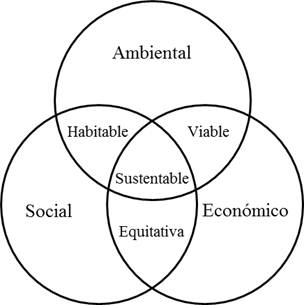
\includegraphics[width=0.3\textwidth]{Figura2}
\end{center}
\begin{center}
\vskip -0.5cm
\caption{\small{Aspectos claves para el desarrollo sustentable.}}
{\small{Fuente: \cite{Tanguay}}}
\end{center}
\end{figure}


\vskip 0.4cm
{\bf Otros ejemplos de antecedentes}: \par

En los años 90 se presentaron definiciones generales las cuales vienen siendo mejoradas. \cite{Dekker} presenta una mejora en la definición de logística reversa como  ”el proceso de planificación, implementación y control de los flujos de materias-primas, en procesos de inventarios y bienes acabados, desde el punto de fabricación, distribución o uso, hacia el punto de recuperación o de eliminación”. 


\begin{figure}[ht]
\begin{center}
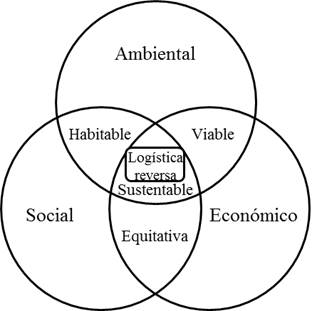
\includegraphics[width=0.3\textwidth]{Figura1}
\end{center}
\begin{center}
\vskip -0.5cm
\caption{\small{Logística reversa incluida en el desarrollo sustentable.}}
{\small{Fuente: Adaptación de \cite{Tanguay}}}
\end{center}
\end{figure}



\vskip 0.4cm
El problema de ruteo de vehículos \citep{Ombuki, Yeun} y sus variantes han ganado mucho interés en la comunidad académica. La intención de estar más cerca a la realidad mediante el modelamiento matemático, hace que se hayan desarrollado nuevos modelos de optimización. \par
\vskip 0.4cm
Según \cite{Sterle} el primer nivel de la red comprende la distribución de la carga desde las plataformas hasta las unidades satélites, utilizando vehículos de carga de mayor tamaño (g).  El segundo nivel, consiste en montar rutas desde las unidades satélites hasta los clientes, usando para este caso vehículos de menor tamaño (v). El modelo de localización y ruteo de vehículos para la distribución de carga propuesto por el autor, además de hacer la conexión de los dos niveles y estudiar su inter relación y dependencia, el modelo busca determinar la cantidad necesaria de plataforma y de unidades satélites considerando el tamaño y dimensionamiento de la flota para el ruteo en dos niveles. 
\vskip 0.2cm


\begin{table}[h!]
\begin{center}
\caption{\small{Resultados computacionales obtenidos en el modelo de \cite{Sterle}}}
\end{center}
\vskip -0.7cm
\begin{tabular}{cccc} \toprule %{|c|c|c|c|} \toprule
\hline 
\rowcolor{LightBlue2}{\small Escenarios} & {\small Demanda cliente (ton.)} & {\small Tiempo (min.)} & {\small Costo ($\$$)} \\ \hline 
{\small 1} & {\small P1:1; P2:2; P3:2; P4:2; P5:1} & {\small 0.12} & {\small 667.42} \\ \hline 
{\small 2} & {\small P1:1; P2:2; P3:2; P4:2; P5:1; P:4; P7:3} & {\small 56.54} & {\small 1744.35} \\ \hline 
{\small 3} & {\small P1: 1; P2:2; P3:2; P4:2; P5:1; P6: 4; P7:3; P8:2; P9:2} & {\small 287.70} & {\small 1750.72} \\  \hline 
{\small 4} & {\small P1:1; P2:2; P3: 2; P4:2; P5:1; P6:4; P7:3; P8:2; P9:2; P10:1} & {\small 1848.57} & {\small 1773.46} \\   \bottomrule \hline 
\end{tabular} 
\begin{center}
\vskip -0.2cm
{\small{Fuente: Resultados obtenidos con CPLEX.}}
\end{center}
\end{table}



\subsection{Justificación}
La mayoría de las investigaciones se efectúan con un propósito definido. Tal propósito debe ser lo suficientemente fuerte para que justifique su realización. \cite{Erica}  

\begin{enumerate}
\item[(a)] Razones o motivos e importancia del tema a ser investigado. 
\item[(b)]Sustentar la pertinencia de la pregunta o problema que se abordará en la investigación.
\item[(c)]Considerar los resultados esperados e impactos previstos.
\end{enumerate}


\subsection{Problema}
Plantear el problema no es otra cosa mas que afinar y estructurar formalmente la idea de investigación. El planteamiento del problema puede ser sencillo o complejo dependiendo de la familiarización del investigador en el tema a tratar.\par    
\vskip 0.3cm
Los criterios para formular un problema de investigación son:
\begin{enumerate}
\item[a)] El problema debe ser formulado claramente y sin ambiguedad como pregunta: ¿Qué efecto?; ¿en qué condiciones ...?; ¿cuál es la probabilidad de ...?; ¿cómo se relaciona ... con ...?; ¿cómo ...?.
\vskip 0.3cm
\item[b)] El planteamiento debe implicar la posibilidad de realizar una prueba empírica o una recolección de datos, es decir, la factibilidad de observarse en la realidad o en un entorno. 
\end{enumerate}
Por lo tanto, los elementos para plantear un problema de investigación son tres y estan relacionados entre si: Los objetivos que persigue la investigación; las preguntas de investigación y la justificación del estudio. \cite{Erica}
\vskip 0.3cm
{\bf Ejemplo:}\par  
¿Cómo viabilizar una red logística reversa en regiones urbanas minimizando los costos logísticos de ruteo y transporte de los RSU hasta su disposición final?


\subsection{Hipótesis}
Preferentemente para investigaciones explicativas debe ser una respuesta a priori y tentativa guardando coherencia con el problema científico, se formula como una proposición afirmativa, con un lenguaje claro y específico.  Las hipótesis se obtienen por deducción lógica y está sustentada en los conocimientos científicos. \par  
\vskip 0.3cm
{\bf Criterios para formular hipótesis:} \cite{Erica}
\begin{enumerate}
\item[a)] Toda hipótesis de investigación debe ser verificable estadísticamente.  Puede ser difícil o imposible de verificar porque no existe un conocimiento sobre el cual se pueda formular una hipótesis, o bien, porque una o más variables no son medibles.
\vskip 0.2cm
\item[b)] Toda hipótesis debe indicar la relación entre variables, lo que implica que las variables deben ser medibles.
\vskip 0.2cm
\item[c)] Toda hipótesis debe tener sus límites. Pueden escogerse hipótesis que sean sencillas de validar, y sin embargo, altamente significativas.
\vskip 0.2cm
\item[d)] El investigador debe tener una razón específica para considerar una hipótesis, ya sea teórica o por alguna evidencia concreta.    
\end{enumerate}


\subsection{Variables}
{\bf Hipótesis:} Existe un mayor número de plantas comestibles en climas cálidos que en climas fríos. \par 
\vskip 0.2cm
Los elementos que se están relacionando son: \par 
\begin{enumerate} [(1)]
	\item  plantas comestibles
	\item  climas cálidos
	\item[(3)] climas fríos
\end{enumerate} 
Estos tres elementos son variables.

\vskip 0.2cm  
\subsubsection{Variable independiente}
Los climas.

\subsubsection{Variables dependiente}
Plantas comestibles.
\vskip 0.3cm


\subsection{Objetivos}

\subsubsection{Objetivos generales}

\begin{enumerate}[a)]%for small alpha-characters within brackets.
	\item Desarrollar un algoritmo de aprendizaje no supervisado para predecir la respuesta correcta de una pregunta de opción múltiple.
\end{enumerate}


\subsubsection{Objetivos específicos}
\begin{enumerate}[a)]
\item Codificar el algoritmo de aprendizaje no supervisado para trabajar con clusters.
\item Desarrollar del prototipo de software y aplicarla a la predicción de la respuesta correcta.
\item Realizar las pruebas y documentar resultados.
\end{enumerate}



\subsection{Método de trabajo}


\vskip 0.1cm
Para llegar a los objetivos propuestos, el desarrollo de la investigación comprendió las siguientes etapas de trabajo a saber:
\begin{enumerate} [a)]
\item Formulación del problema principal de la investigación, justificando su importancia.
\item Búsqueda del material bibliográfico de los diferentes temas necesarios para la elaboración de la investigación, tales como aprendizaje automático no supervisado, probabilidades,estadísticas, desarrollo web, entre otros.
\item Estudio y análisis de los algoritmos de aprendizaje automático no supervisado.
\item Estudio de modelos probabilísticos y estadísticos que contribuyan con el tema de predicciones.
\item Desarrollo del algoritmo de aprendizaje automático no supervisado.
\item Desarrollo del prototipo de software web.
\item Elección de los datos de prueba.
\item Testear, validar y documentar los resultados de la investigación
\end{enumerate}
   


\subsection{Referencias}
Presentar bibliografía conforme a las normas técnicas internacionales reconocidas: Un solo estilo American Psychological Association - APA. Seguir exactamente la forma de las referencias dadas como ejemplos. No usar numeros entre corchetes. Ver los ejemplos de las referencias dadas abajo.\par
\vskip 0.3cm
Se exige como mínimo 10 referencias entre libros y/o artículos referentes al tema a investigar. Las referencias sustentan la investigación del TG.

\bibliography{Bibliografia} % Bibliografia formato APA


\vskip 1cm

\hspace{0.7cm}Edgar\hspace{.1cm}M.\hspace{.1cm} Peche\hspace{.1cm}Perlado 
\hspace{4cm}Manuel\hspace{.1cm}E.\hspace{.1cm} Pérez\hspace{.1cm}Yon \\
\hspace*{2.6cm} Alumno  \hspace*{6.6cm}Alumno


\vskip 1cm
\begin{center}
Alan \hspace{.1cm}M.\hspace{.1cm} Turing\hspace{.1cm}Godel\\
 Asesor
\end{center}



\end{document}

